\section{State-based assertions on fluents\label{section:background-fluents}}

Miller and Shanahan define fluents as ``\emph{time-varying properties of the world that are true at particular time-points if they have been initiated by an event occurrence at some earlier time-point, and not terminated by another event occurrence in the meantime. Similarly, a fluent is false at a particular time-point if it has been previously terminated and not initiated in the meantime}''~\cite{Miller:2002}.

Fluents will allow us to integrate event-based and state-based specification styles within a simple framework~\cite{Giannakopoulou:2003}. 

A fluent $Fl$ is thus a proposition defined by a set $Init_{Fl}$ of initiating events, a set $Term_{Fl}$ of terminating events, and an initial value $Initially_{Fl}$ that can be true or false. The sets of initiating and terminating events must be disjoint. The concrete syntax for fluent definitions is the following~\cite{Giannakopoulou:2003}:

\begin{center}
fluent $Fl = \textless Init_{Fl}, Term_{Fl} \textgreater $ initially $Initially_{Fl}$
\end{center}

In our train example, the safety goal ``\emph{\texttt{Doors shall remain closed while the train is moving}}'' suggests two fluents defined as follows:

\begin{center}
fluent $Moving = \textless \{start\}, \{stop\} \textgreater $ initially \emph{false} \\
fluent $DoorsClosed = \textless \{close\}, \{open\} \textgreater $ initially \emph{true} \\
\end{center}

\subsection{Fluent values along single traces\label{subsection:background-fluents-single-traces}}

In terms of our trace semantics, a fluent $Fl$ will be \emph{true} after a finite trace $s$ if and only if one of the following conditions hold~\cite{Giannakopoulou:2003}:

\begin{enumerate}
\item $Fl$ holds initially and no terminating event has occurred in $s$.
\item Some initiating event has occurred in $s$ with no terminating event occurring since then.
\end{enumerate}

As sets of initiating and terminating events are disjoint, the value of a fluent after a given trace is deterministic. 

For example, the fluent \emph{Moving} is \emph{true} after the trace \artifact{<start stop start>}, but not after the empty trace $\lambda$ nor after \artifact{<start stop>}. 

As prefixes of traces are also traces, we may also think in terms of fluent values \emph{along} traces. This is illustrated in Fig.~\ref{image:fluent-values-along-a-trace} where the values of the two fluents introduced above are shown in the states of a LTS capturing a typical event trace for the train system. 

\begin{figure}[H]\centering
\scalebox{0.41}{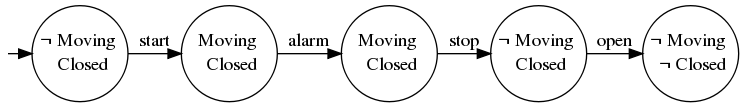
\includegraphics{src/2-framework/images/decorating-trace}}
\caption{LTS annotated with fluent values along a single trace (\artifact{Closed} is an abbreviate for \artifact{DoorsClosed}).\label{image:fluent-values-along-a-trace}}
\end{figure}

As the example suggests, for a set of fluents $\Phi$, an event trace yields an interpretation over $2^\Phi$, that is, an assignment of a Boolean value to each fluent in $\Phi$. We will call it \emph{fluent value assignment} throughout the thesis. 

For example, the maximal trace \artifact{<start alarm stop open>} in Fig.~\ref{image:fluent-values-along-a-trace} yields the following fluent value assignment:
\begin{center}
\{\emph{Moving} $=$ \emph{false}, \emph{DoorsClosed} $=$ \emph{false}\}
\end{center}

\subsection{Fluent values along multiple traces}

We can similarly annotate the states of any LTS. The generalization consists in considering that a LTS state may be reached by a set of traces instead of a single one. Annotations therefore become \emph{sets} of fluent assignments, that is elements of the powerset $\mathcal{P}(2^\Phi)$ over $2^\Phi$. 

In particular, a state might be reached by a trace yielding a fluent \emph{true}, while another trace reaching it would yield the same fluent \emph{false}. Note that even in presence of a possibly infinite number of traces, the set of all possible annotations is itself finite. 

$\mathcal{P}(2^\Phi)$ actually coincides with the set of propositional formulas over fluents. In fact, it appears convenient to consider state annotations as such formulas, where \emph{false} then corresponds to an empty set of fluent assignments (i.e. an unreachable state) and \emph{true} corresponds to the set of all possible assignments. Such state annotations will be called \emph{state invariants}; they encode assertions that always hold when the LTS state is visited. 

Fig.~\ref{image:fluent-values-along-multiple-traces} shows an example of LTS annotated with state invariants.

\begin{figure}[H]\centering
\scalebox{0.41}{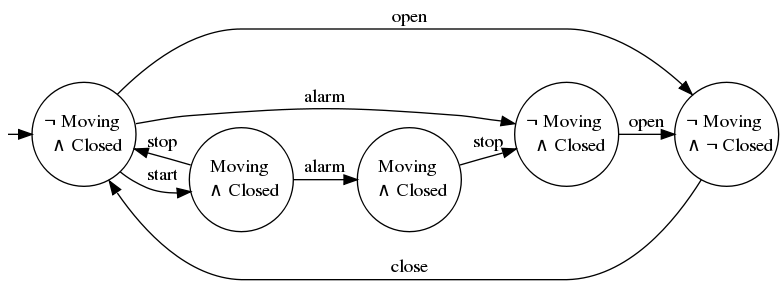
\includegraphics{src/2-framework/images/decorating-lts}}
\caption{Fluent values along multiple traces (\artifact{Closed} is an abbreviate for \artifact{DoorsClosed}).\label{image:fluent-values-along-multiple-traces}}
\end{figure}

A fixpoint algorithm for decorating LTS with fluent value assignments appeared in~\cite{Damas:2005}. This algorithm was generalized for generating weakest state invariants in \cite{Damas:2009}. Very roughly, it consists in annotating the LTS initial state with an initial invariant according to fluent initial values; invariants are then propagated along LTS transitions, according to fluent definitions, and accumulated in states through Boolean disjunction, until a fixpoint is reached. 

Binary decision diagrams~\cite{Bryant:1986} can be used for concisely encoding and efficiently manipulating Boolean formulas (see Chapter~\ref{chapter:tool-support}). This algorithm has been further generalized in~\cite{Damas:2011} for handling other kinds of decorations than state invariants.

\subsection{Integrating fluents in multi-view models}

Fluents provide a general mechanism for integrating event-based and state-based specifications. We will use them for integrating agents, their state machines, and scenarios. The next section extends such integration by introducing fluent-based goals and domain properties.

We will restrict our use of fluents to the ones that are monitorable and controllable by the agents forming the system~\cite{Letier:2002}. 

A fluent is \emph{monitorable} by an agent if all its initiating and terminating events can be either sent or received by this agent. It is \emph{controllable} if all initiating and terminating events can be sent by the agent. 

Our restriction to fluents that are monitorable or controllable by system agents is motivated by the need for specifications  to be realizable by the agents involved in them~\cite{Letier:2002}.
